%%% The main file. It contains definitions of basic parameters and includes all other parts.

%% Settings for single-side (simplex) printing
% Margins: left 40mm, right 25mm, top and bottom 25mm
% (but beware, LaTeX adds 1in implicitly)
\documentclass[12pt,a4paper]{report}
\setlength\textwidth{145mm}
\setlength\textheight{247mm}
\setlength\oddsidemargin{15mm}
\setlength\evensidemargin{15mm}
\setlength\topmargin{0mm}
\setlength\headsep{0mm}
\setlength\headheight{0mm}
% \openright makes the following text appear on a right-hand page
\let\openright=\clearpage

%% Settings for two-sided (duplex) printing
% \documentclass[12pt,a4paper,twoside,openright]{report}
% \setlength\textwidth{145mm}
% \setlength\textheight{247mm}
% \setlength\oddsidemargin{14.2mm}
% \setlength\evensidemargin{0mm}
% \setlength\topmargin{0mm}
% \setlength\headsep{0mm}
% \setlength\headheight{0mm}
% \let\openright=\cleardoublepage

%% Prefer Latin Modern fonts
\usepackage{lmodern}

%% Further useful packages (included in most LaTeX distributions)
\usepackage{amsmath}        % extensions for typesetting of math
\usepackage{amsfonts}       % math fonts
\usepackage{amsthm}         % theorems, definitions, etc.
\usepackage{bbding}         % various symbols (squares, asterisks, scissors, ...)
\usepackage{bm}             % boldface symbols (\bm)
\usepackage{graphicx}       % embedding of pictures
\usepackage{fancyvrb}       % improved verbatim environment
\usepackage{natbib}         % citation style AUTHOR (YEAR), or AUTHOR [NUMBER]
\usepackage[nottoc]{tocbibind} % makes sure that bibliography and the lists
			    % of figures/tables are included in the table
			    % of contents
\usepackage{dcolumn}        % improved alignment of table columns
\usepackage{booktabs}       % improved horizontal lines in tables
\usepackage{paralist}       % improved enumerate and itemize
\usepackage[usenames, table]{xcolor}  % typesetting in color


\usepackage[colorinlistoftodos,prependcaption,textsize=tiny]{todonotes}
\usepackage{xargs}
\newcommandx{\unsure}[2][1=]{\todo[linecolor=red,backgroundcolor=red!25,bordercolor=red,#1]{#2}}
\newcommandx{\change}[2][1=]{\todo[linecolor=blue,backgroundcolor=blue!25,bordercolor=blue,#1]{#2}}
\newcommandx{\info}[2][1=]{\todo[linecolor=OliveGreen,backgroundcolor=OliveGreen!25,bordercolor=OliveGreen,#1]{#2}}
\newcommandx{\improvement}[2][1=]{\todo[linecolor=Plum,backgroundcolor=Plum!25,bordercolor=Plum,#1]{#2}}
\newcommandx{\thiswillnotshow}[2][1=]{\todo[disable,#1]{#2}}

\usepackage{enumitem}

%% Generate PDF/A-2u
\usepackage[a-2u]{pdfx}

%% Character encoding: usually latin2, cp1250 or utf8:
\usepackage[utf8]{inputenc}

\usepackage{hyperref}


%%% Basic information on the thesis

%%% XXX TODO
\title{HexMage}

% Thesis title in English (exactly as in the formal assignment)
\def\ThesisTitle{Using procedural content generation to balance encounters in RPG-like games}

% Author of the thesis
\def\ThesisAuthor{Jakub Arnold}

% Year when the thesis is submitted
\def\YearSubmitted{2017}

% Name of the department or institute, where the work was officially assigned
% (according to the Organizational Structure of MFF UK in English,
% or a full name of a department outside MFF)
\def\Department{Department of Software and Computer Science Education}

% Is it a department (katedra), or an institute (ústav)?
\def\DeptType{Department}

% Thesis supervisor: name, surname and titles
\def\Supervisor{Mgr. Jakub Gemrot}

% Supervisor's department (again according to Organizational structure of MFF)
\def\SupervisorsDepartment{Department of Software and Computer Science Education}

% Study programme and specialization
\def\StudyProgramme{Computer Science}
\def\StudyBranch{Programming and Software Systems}

% An optional dedication: you can thank whomever you wish (your supervisor,
% consultant, a person who lent the software, etc.)
\def\Dedication{%
Dedication.
}

% Abstract (recommended length around 80-200 words; this is not a copy of your thesis assignment!)
\def\Abstract{%
Procedural content generation (PCG) is mostly examined in the context of
map/environment creation, rather than generating the actual game characters.
The goal of this thesis is to design a turn-based RPG-like game with perfect information
for which we can generate balanced encounters. The game consists of a hex-based arena
in which two teams fight. Each team consists of a few player controller characters
with unique abilities. We generate the attributes of these abilities in order
to make the encounter balanced. We will also build an AI that
can be used to automatically play-test the PCG algorithm. The goal is to generate an equally
strong, but different opponent.}

% 3 to 5 keywords (recommended), each enclosed in curly braces
\def\Keywords{%
{video games} {encounter balancing} {hex arena} {rpg elements}
}

%% The hyperref package for clickable links in PDF and also for storing
%% metadata to PDF (including the table of contents).
%% Most settings are pre-set by the pdfx package.
\hypersetup{unicode}
\hypersetup{breaklinks=true}

% Definitions of macros (see description inside)
%%% This file contains definitions of various useful macros and environments %%%
%%% Please add more macros here instead of cluttering other files with them. %%%

%%% Minor tweaks of style

% These macros employ a little dirty trick to convince LaTeX to typeset
% chapter headings sanely, without lots of empty space above them.
% Feel free to ignore.
\makeatletter
\def\@makechapterhead#1{
  {\parindent \z@ \raggedright \normalfont
   \Huge\bfseries \thechapter. #1
   \par\nobreak
   \vskip 20\p@
}}
\def\@makeschapterhead#1{
  {\parindent \z@ \raggedright \normalfont
   \Huge\bfseries #1
   \par\nobreak
   \vskip 20\p@
}}
\makeatother

% This macro defines a chapter, which is not numbered, but is included
% in the table of contents.
\def\chapwithtoc#1{
\chapter*{#1}
\addcontentsline{toc}{chapter}{#1}
}

% Draw black "slugs" whenever a line overflows, so that we can spot it easily.
\overfullrule=1mm

%%% Macros for definitions, theorems, claims, examples, ... (requires amsthm package)

\theoremstyle{plain}
\newtheorem{thm}{Theorem}
\newtheorem{lemma}[thm]{Lemma}
\newtheorem{claim}[thm]{Claim}

\theoremstyle{plain}
\newtheorem{defn}{Definition}

\theoremstyle{remark}
\newtheorem*{cor}{Corollary}
\newtheorem*{rem}{Remark}
\newtheorem*{example}{Example}

%%% An environment for proofs

%%% FIXME %%% \newenvironment{proof}{
%%% FIXME %%%   \par\medskip\noindent
%%% FIXME %%%   \textit{Proof}.
%%% FIXME %%% }{
%%% FIXME %%% \newline
%%% FIXME %%% \rightline{$\square$}  % or \SquareCastShadowBottomRight from bbding package
%%% FIXME %%% }

%%% An environment for typesetting of program code and input/output
%%% of programs. (Requires the fancyvrb package -- fancy verbatim.)

\DefineVerbatimEnvironment{code}{Verbatim}{fontsize=\small, frame=single}

%%% The field of all real and natural numbers
\newcommand{\R}{\mathbb{R}}
\newcommand{\N}{\mathbb{N}}

%%% Useful operators for statistics and probability
\DeclareMathOperator{\pr}{\textsf{P}}
\DeclareMathOperator{\E}{\textsf{E}\,}
\DeclareMathOperator{\var}{\textrm{var}}
\DeclareMathOperator{\sd}{\textrm{sd}}

%%% Transposition of a vector/matrix
\newcommand{\T}[1]{#1^\top}

%%% Various math goodies
\newcommand{\goto}{\rightarrow}
\newcommand{\gotop}{\stackrel{P}{\longrightarrow}}
\newcommand{\maon}[1]{o(n^{#1})}
\newcommand{\abs}[1]{\left|{#1}\right|}
\newcommand{\dint}{\int_0^\tau\!\!\int_0^\tau}
\newcommand{\isqr}[1]{\frac{1}{\sqrt{#1}}}

%%% Various table goodies
\newcommand{\pulrad}[1]{\raisebox{1.5ex}[0pt]{#1}}
\newcommand{\mc}[1]{\multicolumn{1}{c}{#1}}


% Title page and various mandatory informational pages
\begin{document}
%%% Title page of the thesis and other mandatory pages

%%% Title page of the thesis

\pagestyle{empty}
\hypersetup{pageanchor=false}
\begin{center}

\centerline{\mbox{
\includegraphics[width=166mm]{img/logo-en.pdf}}}

\vspace{-8mm}
\vfill

{\bf\Large BACHELOR THESIS}

\vfill

{\LARGE\ThesisAuthor}

\vspace{15mm}

{\LARGE\bfseries\ThesisTitle}

\vfill

\Department

\vfill

\begin{tabular}{rl}

Supervisor of the bachelor thesis: & \Supervisor \\
\noalign{\vspace{2mm}}
Study programme: & \StudyProgramme \\
\noalign{\vspace{2mm}}
Study branch: & \StudyBranch \\
\end{tabular}

\vfill

% Zde doplňte rok
Prague \YearSubmitted

\end{center}

\newpage

%%% Here should be a bound sheet included -- a signed copy of the "bachelor
%%% thesis assignment". This assignment is NOT a part of the electronic
%%% version of the thesis. DO NOT SCAN.

%%% A page with a solemn declaration to the bachelor thesis

\openright
\hypersetup{pageanchor=true}
\pagestyle{plain}
\pagenumbering{roman}
\vglue 0pt plus 1fill

\noindent
I declare that I carried out this bachelor thesis independently, and only with the cited
sources, literature and other professional sources.

\medskip\noindent
I understand that my work relates to the rights and obligations under the Act No.~121/2000 Sb.,
the Copyright Act, as amended, in particular the fact that the Charles
University has the right to conclude a license agreement on the use of this
work as a school work pursuant to Section 60 subsection 1 of the Copyright Act.

\vspace{10mm}

\hbox{\hbox to 0.5\hsize{%
In ........ date ............	% FIXME!
\hss}\hbox to 0.5\hsize{%
signature of the author
\hss}}

\vspace{20mm}
\newpage

%%% Mandatory information page of the thesis

\openright

\vbox to 0.5\vsize{
\setlength\parindent{0mm}
\setlength\parskip{5mm}

Title:
\ThesisTitle

Author:
\ThesisAuthor

\DeptType:
\Department

Supervisor:
\Supervisor, \SupervisorsDepartment

Abstract:
\Abstract

Keywords:
\Keywords

\vss}

\newpage

%%% Dedication

\openright

\noindent
\Dedication

\newpage

\openright
\pagestyle{plain}
\pagenumbering{arabic}
\setcounter{page}{1}


%%% A page with automatically generated table of contents of the bachelor thesis

\tableofcontents

%%% Each chapter is kept in a separate file
\chapwithtoc{Introduction}

An increasing number of computer games is using procedural content generation
(PCG) as one of their core mechanics. This is in different contexts, most
commonly for generating new levels (e.g. \citet{diablo}). \todo{zobrazovat nazev a ne autora} Occasionally games
even generate player collectible items (e.g. \citet{borderlands}). However,
there has not been much research on the use of procedural generation for
balancing encounters in RPG games. By this we mean procedurally generating
enemies that can be defeated by the player, but pose a challenge. A crucial
criteria here is that the balance is not simply achieved by creating the enemy
as an exact clone of the player, but rather explore the search-space to find an
enemy that is not only balanced, but also different from the player.

One particular application for this kind of PCG is automatic difficulty
adjustments based on the player's skill. Another possible use could be
automatic generation of new and unique enemies based on given constraints,
which is the approach we chose in this thesis.

We have created a custom game with mechanics that are simple enough to simulate
quickly, yet flexible enough to represent a large search space. There are two
teams that fight in a hexagonal arena, each consists of a small number of
player controlled characters (mages), and each mage has a small number of
abilities. In each turn the player has control over one of his characters, and
both move around the map and cast spells, in any order he wishes. The only
limit is the number of action points the character has available, which are
consumed both by movement and ability usage. The side that first eliminates the
opposing team wins.

All information is visible to all players, and all actions are completely
deterministic. There is no time limit for the player action, which means the
player could theoretically calculate a perfect move given enough time.

The goal of this thesis is to explore PCG options for balancing encounters in
turn-based RPG-like games. We design a simple game with flexible mechanics, and
build an AI that can be used to approximate the player. We then use evolution strategies
to generate opponents of just the right difficulty for the given player team, using AI vs
AI combat as a fitness function.

\subsection*{Organization}

In Chapter 1 we begin by defining the scope of the work, our general approach,
and list related work. Chapter 2 follows by exploring our game mechanics in
detail and explaining the choices behind them. Next in Chapter 3 we will go
over our different choices for implementing the AI.

Chapter 4 describes our approach to generating the encounters, with the expriments
described in Chapter 5 and a conclusion in Chapter 6. Lastly, the Appendix contains
programmer documentation with implementation details.

% \part{Analysis}
\chapter{Problem Definition}

\section{Game types}

\section{Types of PCG currently being used}

\section{Our game}

- game that can generalize to real life scenarios
- simple mechanics that are representative
- fast to simulate


Two teams fight on a hexagonal map (\emph{arena}) of small size (radius of
5-10 hexes). Each team consists of a small number of player controller
characters (\emph{mages} for short), and each mage has a small number of
\emph{abilities}, \emph{health}, and \emph{action points}. Players take turns, during
which each player has control over one of his mages. The player can issue
commands to move around the arena and use abilities. Both movement and ability
usage costs action points, which are restored at the end of the turn.  Moving
one hex costs one action point. The cost of using an ability varies, and is one
of the parameters that we optimize for when looking for a balanaced game. An
ability can also have a \emph{cooldown}, which prevents repeated usage for a
given number of turns \todo{znovu rozlisovat turn}. Note that the cooldown can
be zero, which means the ability can be used multiple times per turn
\todo{turn}.

\missingfigure{obrazek areny?}

Abilities can do direct damage to an enemy mage, apply a \emph{debuff} (causing
damage and decreasing action points over time), and create an area of effect
(\emph{AOE}) debuff that spans multiple hexes in the arena. Both the debuffs and
AOEs are applied at the end of each turn \todo{rozlisovat turn maga a turn hry
(round?)}, which happens after both players finish playing all their mages.
Both debuffs and AOEs also have a lifetime, which specifies how many turns
\todo{znova turn} the effect lasts.

% \part{Implementation}
\chapter{Game Rules and Mechanics}
\label{chapter02}

Two teams fight on a hexagonal map (\emph{arena}) of small size (radius of
5--10 hexes, see \autoref{fig:arena}). The map contains empty hexes and walls.
Each team consists of a small number of player controller
characters (\emph{mages} for short), and each mage has a small number of
\emph{abilities}, \emph{health}, and \emph{action points}. Players take turns, during
which each player has control over one of his mages. The player can issue
commands to move around the arena and use abilities. Mages can only walk on empty hexes
and cannot cast through walls.

There is also an important distinction between a \emph{turn} and a \emph{round}.
A turn means playing all the actions a single mage can do with his action points,
and ends when the player decides he is finished playing with that one single character.
A round ends when all of the characters have played their turn, and it is at that point
when debuffs, AOEs, cooldowns and action points are re-calculated (see below).

Both movement and ability usage costs action points, which are restored at the
end of the round. Moving one hex costs one action point. The cost of using an
ability varies, and is one of the parameters that we optimize for when looking
for a balanaced game. An ability can also have a \emph{cooldown}, which
prevents repeated usage for a given number of rounds. Note that the cooldown
can be zero, which means the ability can be used multiple times per turn.
Abilities also have limited range, which supports positional gameplay.

Abilities can do direct damage to an enemy mage, apply a \emph{debuff} (causing
damage and decreasing action points over time), and create an area of effect
(\emph{AOE}) debuff that spans multiple hexes in the arena. Both the debuffs and
AOEs are applied at the end of each round. Both debuffs and AOEs also have a lifetime,
which specifies how many rounds the effect lasts.

The motivation for having cooldowns is that it allows us to generate powerful
abilities that don't necessarily take up the whole turn of the player by costing
a lot of action points. If the ability is cheap, but has a large cooldown, it can
serve a strategic purpose, as the player might want to prepare his position in order
to use the ability when the cooldown wears off. AOE abilities also improve positional
gameplay, as they can be used to force the enemy player to move out of position.

\begin{figure}[h]
	\centering
	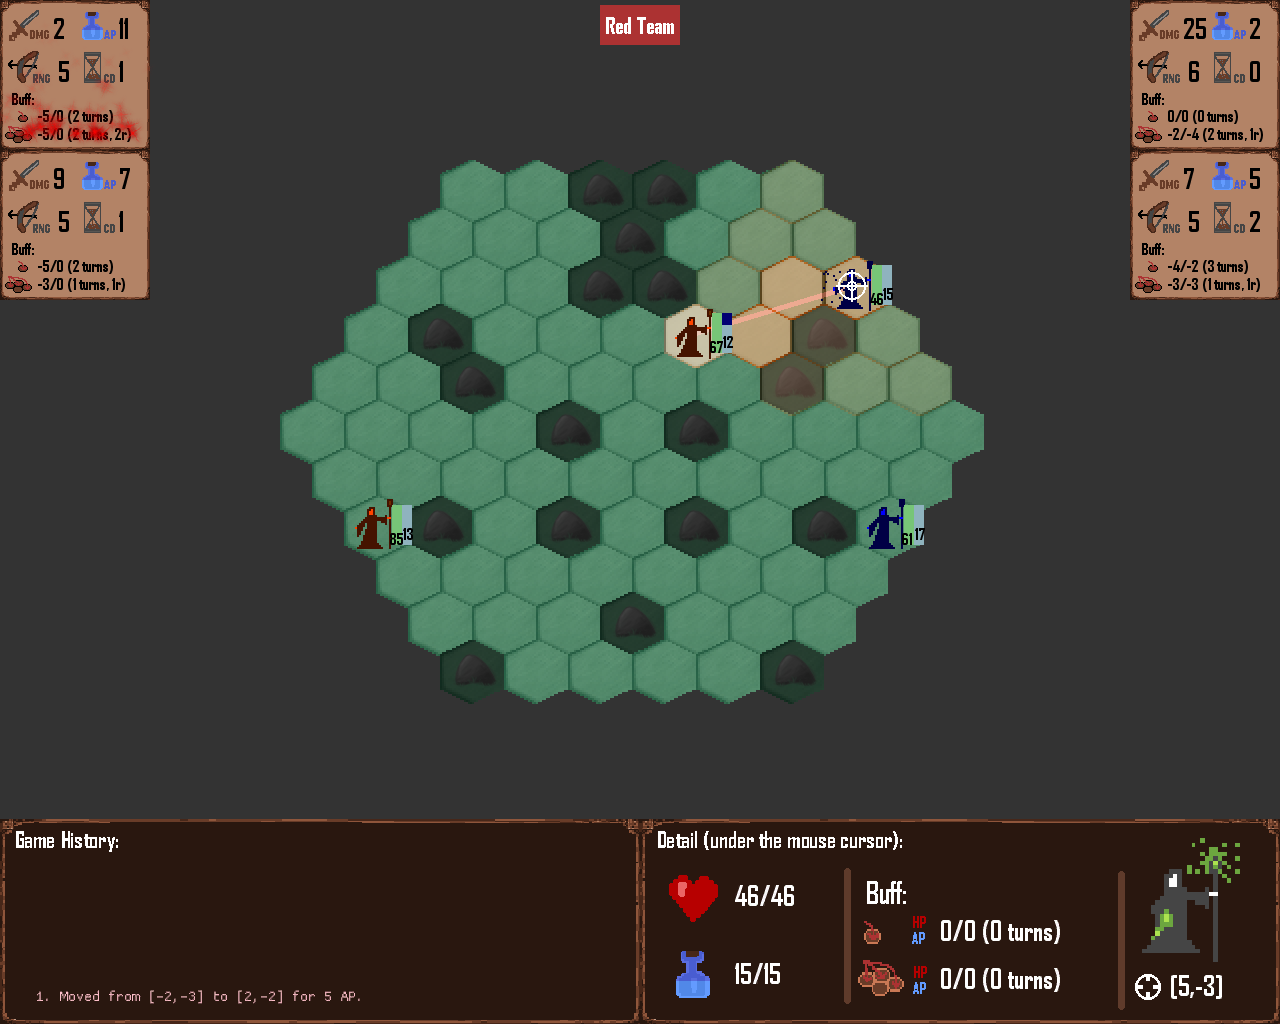
\includegraphics[width=0.95\textwidth]{img/arena.png}
	\caption{User interface of the HexMage game, featuring a 2v2 game. The red player currently has a spell selected and is targeting one of the blue player's mages.}
	\label{fig:arena}
\end{figure}


\section{Simulator}

Part of our game is a simulator that can be used as a library and encapsulates
all of the game rules and mechanics. This is then used by both the AI and the
PCG algorithm and can thus be run separately from the main game. The game is
internally represented by a \emph{state} object, and all of the possible player
actions are encapsulated by an \emph{action} object.  Playing the game through
the library then simply becomes a matter of applying a state transition
function $f: (\text{state}, \text{action}) \rightarrow \text{state}$.

Here's a list of all possible actions at an arbitrary state:

\begin{description}
\item [AbilityUse] Use an ability targeting an enemy that is already in range.
\item [Move] Move the current mage to a different hex on the map.
\item [EndTurn] Finish the current turn.
\item [DefensiveMove] Serves the same purpose as \emph{Move}, but carries an
additional information in the sense that \emph{DefensiveMove} can only be
the last action of the turn.
\item [AttackMove] Combines the \emph{Move} and \emph{AbilityUse} actions into one.
\item [NullAction] Doesn't do anything and is mostly used as a placeholder in cases no action is possible.
\end{description}

The simulator also verifies that no invalid actions are applied through a
thorough list of invariant checks. These are automatically turned off in a
release build to make the simulator run as fast as possible.

The simulator is also built to be high performance and can easily run hundreds
of thousands to millions of actions per second on a consumer-grade PC\@.
The state object is split into two parts, one that handles the
general immutable information that doesn't change as the game progresses (i.e.\
max hitpoints, ability definitions, etc.), and one that handles all of the
mutable data, such as current hitpoints, current positions on the map, etc.
This allowed us to make state copies very fast as well, running only at a few
microseconds per copy.

\chapter{Generating Encounters}

We approach generating encounters as a search based problems with two
different approaches, Simulated Annealing and Evolution Strategies. (\todo{reference})

To make the search algorithms as general as possible, we serialize our
internal game representation into a single vector of normalized floating
point values (DNA). The algorithm then doesn't need to understand our game
mechanics and restriction, and can be applied to different configurations of
the game independently.

To avoid balancing via specific attributes, one can simply remove them from
the serialization/deserialization routines that transform the game setup into
the DNA vector, without altering any of the logic for balancing encounters.

In the case of our experiments, we chose to stick with 2v2 games on a fixed map,
where each mage has only two abilities. This was chosen both with respect to our
questionnaire, and running time of the algorithms. Choosing a larger team setup or
a bigger map (or many different maps) would be difficult for the participants,
and would also take much longer to compute our experimental data.

\missingfigure{mapa}

- popsat jak funguje reprezentace DNA

\section{Simulated Annealing and Evolution Strategies}

Our initial implementation of generating the encounters was using Simulated
Annealing (\todo{reference}). However, we had difficulty converging to good
results \todo{fuj, napsat jinak}.

As a result, we ran an experiment to sample the search space at roughly 20 million
different points, and measured the change in fitness in the neighbourhood of each point.
We found that in each point's neighbourhood, there are roughly 5 times more points that have
worse fitness than the ones that are an improvement over the current point. We also found that
most of these downward changes were much steeper between 4-7x than the improving points.

Our suspicion is that this is the main cause of failure of Simmulated Annealing, which simply
fails to find the upward slope.

For this reason we chose to try another approach, specificially Evolution Strategies (\todo{reference})

\section{Choice of the Fitness Function}

In order to evaluate the balance of a matchup, we came up with the following fitness function.

\todo{chybi popis}

During the experiment we encountered multiple ways ES tried to exploit the game
mechanics to maximize the balance fitness function in ways that were
undesirable. One example being when the resulting games end up being short as
the algorithm generates mages with lots of AOE abilities that cover the whole
map in the first turn, resulting in immediate death of all characters.

We balance this by introducing an additional fitness function for game length
in the form of a cumulative normal distribution with $\sigma = 10$ and $\mu =
3$.\unsure{overit jestli to tak fakt je}.  This prevents ES from moving towards
short games.

\chapter{Generating Encounters}
\label{chapter04}

There are many possible attributes that can be generated. We could change the size of each team,
the number of abilities of each mage, starting positions of the map, or even change the positions of the walls.

\section{Reducing the Scope of the Problem}

We chose to reduce the scope by creating a small fixed map on which all encounters will be played and balanced.
We also fix the team size of both teams to 2 mages, and each mage to 2 abilities. While this significantly reduces
the possibilities to achieve balance, there are still a lot of parameters that can be tweaked, as described in the next section.

We also put lower and upper bounds on most of the numeric values of attributes of mages and their abilities. See attached programmer documentation in the \autoref{chap:prog-doc} for more details about how attributes are represented.

\section{Approach}

We approach generating encounters as a search based problems with two different
approaches, Simulated Annealing \citep{ai-modern} and Evolution Strategies
\citep{evolution-strategies}.

To make the search algorithms as general as possible, we serialize our
internal game representation into a single vector of normalized floating
point values (DNA). The algorithm then does not need to understand our game
mechanics and restriction, and can be applied to different configurations of
the game independently.

To avoid balancing via specific attributes, one can simply remove them from
the serialization/deserialization routines that transform the game setup into
the DNA vector, without altering any of the logic for balancing encounters.

In the case of our experiments, we chose to stick with 2v2 games on a fixed map,
where each mage has only two abilities. This was chosen both with respect to our
questionnaire, and running time of the algorithms. Choosing a larger team setup or
a bigger map (or many different maps) would be difficult for the participants,
and would also take much longer to compute our experimental data.

Taking these restrictions into mind, the DNA would then take up $96$ floating point values,
specifically: $$2 \text{ Teams} \times 2 \text{ Mages} \times ( HP + AP + 2 \times \text{AbilitySize}) = 96$$ since $\text{Ability Size} = 11$ as we need to serialize damage, cost, range, cooldown,
debuff (HP damage, AP damage, lifetime), and AOE (debuff + lifetime).

\todo{popsat hillclimbing}

\section{Simulated Annealing}

Our initial implementation of generating the encounters was using Simulated
Annealing \citep{ai-modern}. Simulated annealing works similar to a hill climbing algorithm, except
that instead of always picking the best neighbour, we use a probability distribution.
Neighbours with better fitness have a higher probability, but we might still take a path
downhill. The amount of randomness is controlled by an external variable called temperature (or energy).
As the algorithm progresses, the temperature is slowly reduced and thus allows it to converge.
The main advantage over hill climbing is that simulated annealing does not immediately get stuck in a local optima,
as there is always a chance it will move to a state with lower fitness value.

However, we had difficulty getting good results and the algorithm
almost never converged. As a result, we ran an experiment to sample the search space at roughly 20
million different points, and measured the change in fitness in the
neighbourhood of each point. We found that in each point's neighbourhood,
there are roughly 5 times more points that have worse fitness than the ones
that are an improvement over the current point. We also found that most of
these downward changes were much steeper between 4--7x than the improving
points. Our suspicion is that this is the main cause of failure of
Simmulated Annealing, which simply fails to find the upward slope.

\section{Evolution Strategies}

For this reason we chose to try another approach, specificially Evolution
Strategies (ES) \citep{evolution-strategies}. ES works by taking a random sample of the
neighbourhood of the current value, evaluating the fitness of each of the neighbours, and
moving to a state that is the weighted average of the neighbours with respect to their fitness.
This process is iterated until a state with suitable fitness value is found. In our experiments
we have found this approach to consistently converge much faster than simulated annealing.

ES also yields itself to easy parallelization, especially if the evaluation of the fitness
function is complicated. Since all of the neighbouring samples are completely independent,
they can be evaluated completely in parallel.

\section{Choice of the Fitness Function}

In order to evaluate the balance of a matchup, we evaluated the following three
criteria:

\begin{description}
\item [Balance] Unsurprisingly, part of the fitness function is comparing the
  strength of both teams against each other.  We consider games that end in a
    draw balanced.  If the game doesn't end in a draw, we measure the remaining
    HP percentage of the winner, and the lower it is, the more balanced the
    game was.
\item [Game length] We also put an interval restriction on game length. Ideally
  we'd want the game to last at least 2 rounds.
\item [Team difference] Lastly, since we don't to create balance by making both
  teams identical, we added a third criteria that measures the difference of
    both teams.
\end{description}

The combined fitness function is calculated as the average of the three.
See \hyperref[fig:converging-es]{Figure 4.1} for an example
plot of how the fitness function converges using Evolution Strategies.
It is worth noting here that evaluating the fitness function (the \emph{Balance}
part specifically) is computationally intensive, as it requires the whole game
to be played out till the end. We also do this evaluation using an ensemble average of multiple different AIs.
Specifically, we use both the Rule based AI and MCTS in the \emph{Balance} playout and take their average.
This helps assure that the game is balanced despite multiple playstyles, as both the Rule based AI and MCTS
play differently (see \hyperref[tab:winrates]{Table 5.1} for their comparison). You can see how the fitness function
converges in \hyperref[fig:converging-es]{Figure 4.1}.

\begin{figure}
	\centering
	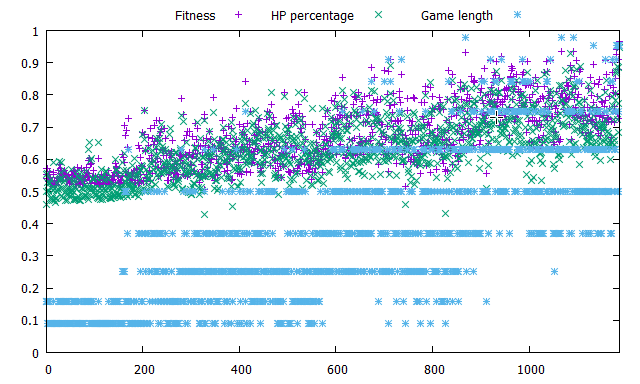
\includegraphics[width=0.75\textwidth]{img/converging-es.png}
	\caption{An exmple of a how the combined fitness function converges over rougly 1200 iterations. Green dots represent the \emph{Balance} fitness measuring HP percentage left at the end of the game, blue dots represent game length, and purple is the combined fitness. We're not showing team difference data points as in this plot.}
	\label{fig:converging-es}	
\end{figure}

\section{Remarks}

During the experiment we encountered multiple ways ES tried to exploit the
game mechanics to maximize the balance fitness function in ways that were
undesirable. One example being when the resulting games end up being short
as the algorithm generates mages with lots of AOE abilities that cover the
whole map in the first turn, resulting in immediate death of all characters.

We balance this by introducing an additional fitness function for game length
in the form of a cumulative normal distribution with mean around $10$ turns.

Lastly, the team difference is measured as an euclidean distance between the DNA
vectors of each team. Again, we use a cumulative normal distribution to put a lower
bound on the team difference.

\chapter{Experiments}
\label{chapter05}

\section{Participants}

The participants were all computer science students. All of them had at least
some experience with computer games, and were presented the mechanics of HexMage
before conducting the experiment.

\section{Experiment Design}

The goal of the experiment is to measure two things. One, if the generated
encounters are actually balanced. And two, if the AI is strong enough to pose a
challenge to the player. We will measure the overall winrate of the players,
and also compare how the AI did in games the player considered balanced.

The experiment consists of 20 different games of HexMage. All of the games are
played on the same map that was hand-designed beforehand. This was to allow the
participants to better get familiar with the game and think ahead. The games
are structured so that each player has 2 mages, each with 2 abilities. This was
to reduce the cognitive overhead for the participants and allow them to more easily
adjust to the 20 completely different scenarios.

The first 10 of the 20 games had the player team hand designed, and the
opponent (played by the AI) generated with our PCG algorithm. The remaining 10
games had both teams generated with no manual tweaks or changes. Having some of
the games hand designed allows us to show that the PCG algorithm can balance
against constraints that aren't completely random. A hand designed team might
have features that are rare in the search space. All of the games are played
against the MCTS based AI\@.

\section{Results}

\missingfigure{korelacni matice}
\missingfigure{grafy}

The results show that most participants consider our MCTS AI to be strong
enough to provide a challengem which is also proven by the 40\% winrate of
the participants. \todo{aktualizovat cisla}

Given the number of played games \todo{overit, ze jich mame dost} we can
rule out the AI having a better setup in most of the scenarios. Based on the
results, around 35\% \todo{aktualizovat cisla} of the games were balanced,
which means in the resulting 65\% one of the players had an advantage.

We consider this result to be positive as the games were generated without
any human intervention and weren't altered before running the experiment.
\todo{link na appendinx s instrukcema na pregenerovani experimentu}

Considering that 35\% of the generated games are balanced, this would allow
the algorithm to be used offline as is to aid design of game levels with
some manual checking of the resulting games.

If one were to design the encounter completely from scratch to be balanced,
it would be very difficult given the number of variables that need to be
optimized.

\section{TODO}

\begin{description}[align=right,labelwidth=3cm]
\item bud zminit ze by to slo delat online s nejaky additional checkem
\item nebo zlepsit fitness aby vyresila patologicke pripady z experimentu?
\end{description}


\chapter{Conclusion and discussion of the results}


%%% Bibliography
%%% Bibliography (literature used as a source)
%%%
%%% We employ bibTeX to construct the bibliography. It processes
%%% citations in the text (e.g., the \cite{...} macro) and looks up
%%% relevant entries in the bibliography.bib file.
%%%
%%% The \bibliographystyle command selects, which style will be used
%%% for references from the text. The argument in curly brackets is
%%% the name of the corresponding style file (*.bst). Both styles
%%% mentioned in this template are included in LaTeX distributions.

\bibliographystyle{plain}    %% Author (year)
% \bibliographystyle{unsrt}     %% [number]

\renewcommand{\bibname}{Bibliography}

%%% Generate the bibliography. Beware that if you cited no works,
%%% the empty list will be omitted completely.

\bibliography{bibliography}

%%% If case you prefer to write the bibliography manually (without bibTeX),
%%% you can use the following. Please follow the ISO 690 standard and
%%% citation conventions of your field of research.

% \begin{thebibliography}{99}
%
% \bibitem{lamport94}
%   {\sc Lamport,} Leslie.
%   \emph{\LaTeX: A Document Preparation System}.
%   2nd edition.
%   Massachusetts: Addison Wesley, 1994.
%   ISBN 0-201-52983-1.
%
% \end{thebibliography}


%%% Figures used in the thesis (consider if this is needed)
\listoffigures

%%% Tables used in the thesis (consider if this is needed)
%%% In mathematical theses, it could be better to move the list of tables to the beginning of the thesis.
\listoftables

%%% Abbreviations used in the thesis, if any, including their explanation
%%% In mathematical theses, it could be better to move the list of abbreviations to the beginning of the thesis.
\chapwithtoc{List of Abbreviations}

%%% Attachments to the bachelor thesis, if any. Each attachment must be
%%% referred to at least once from the text of the thesis. Attachments
%%% are numbered.
%%%
%%% The printed version should preferably contain attachments, which can be
%%% read (additional tables and charts, supplementary text, examples of
%%% program output, etc.). The electronic version is more suited for attachments
%%% which will likely be used in an electronic form rather than read (program
%%% source code, data files, interactive charts, etc.). Electronic attachments
%%% should be uploaded to SIS and optionally also included in the thesis on a~CD/DVD.
%%% Allowed file formats are specified in provision of the rector no. 23/2016.
\chapwithtoc{Attachments}

\openright
\end{document}
